\section{Theoretical background} \label{sec:theory}
This chapter is dedicated to reviewing basic wind turbine theory. Firstly fundamental aerodynamics and airfoil theory is explained. Secondly some basic wind turbine control schemes are shown with regards to different wind-dependent operating regions. Furthermore WT system eigenfrequencies are explained along with the significance of the WT operating speeds with respect to these eigenfrequencies. Fatigue loads are also explained along with how to both calculate and use damage equivalent loads. Finally some FOWT challenges are examined, mainly focused on the negative dampening problem.

\subsection{Aerodynamics and airfoil theory} \label{sec:theory_aero}
The sun delivers energy to the earth by heating up the earths surface and subsequently the air. Winds are created as a result of the pressure differences that occur due to the expansion and contraction of the air. 

WTs work because they are able to convert the wind's energy into a torque in the generator which then generates electrical energy. When the wind blows over the blades of a WT it delivers some of its energy to the blade, yielding both a thrust force and torque to the blade.

In the simplest 1D momentum theory case the delivery of energy just results in a lowing of the wind speed following the rotor area. Due to mass preservation an expansion of the air would follow the rotor area as depicted in \cref{fig:betz}.
\begin{figure}[ht]
	\centering
	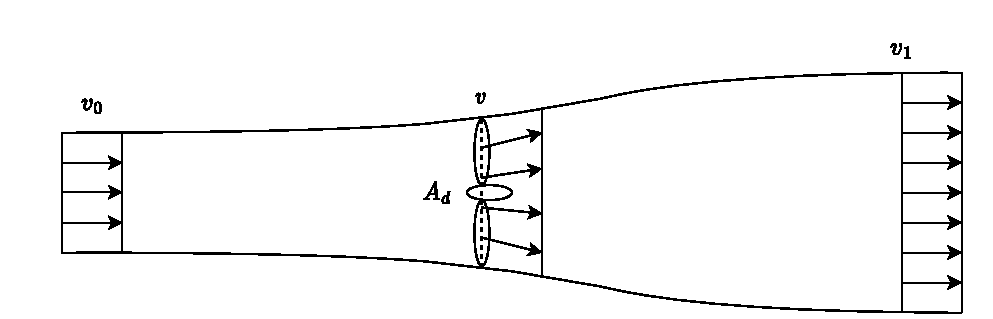
\includegraphics[width=0.8\linewidth]{Graphics/FlowThroughRotor.pdf}
	\caption{Illustration of how a volume of air in a control volume (CV) expands due to a reduction of speed.}
	\label{fig:betz}
\end{figure}

\noindent The power of the \textit{free wind} $ v_0 $ can be expressed from the wind mass flow $ \dot{m} $ through a control volume:
\begin{equation} \label{eq:power}
	P = \dfrac{1}{2} \dot{m} v_0^2
\end{equation}
The flow of mass can be expressed from the air density $ \rho $, the cross sectional area $ A_d $ of the CV at the rotor and the free wind speed $ v_0 $ like so:
\begin{equation}\label{eq:mass_deriv}
	\dot{m} = \rho A_d v_0
\end{equation}
Combining \cref{eq:power} and \cref{eq:mass_deriv} yields:
\begin{equation}\label{eq:power2}
	P_{air} = \dfrac{1}{2} \rho A_d v_0^3
\end{equation}
A \textit{power coefficient} $ C_p $ represents the percentage of the available power that is extracted from the wind:
\begin{equation}\label{eq:Cp}
	C_p = \dfrac{P_T}{P_{air}}
\end{equation}
Such that the extracted power $ P_T $ is defined:
\begin{equation}\label{eq:power_w_Cp}
	P_{T} = \dfrac{1}{2} \rho A_d v_0^3 C_p
\end{equation}
$ C_p $ is dependent on the rotor blade pitch $ \theta $ and the tip speed ratio (TSR) $ \lambda $. In the partial load region the main goal is to reach a maximum $ C_p $ by adjusting $ \theta $ and  $ \lambda $ to their optimal values:
\begin{equation}\label{eq:cp_optimal}
	C_p^\star = C_p(\theta^\star, \lambda^\star)
\end{equation}
Where $ * $ denotes the optimal value of a parameter with regards to $ C_p $ at a given wind speed. This will be further explained in \cref{sec:theory_ctrl}. TSR is the ratio between blade tip speed $ (\Omega R) $ and the incoming free wind speed $v_0$ where $ R $ is the distance from the centre of the rotor and $ \Omega $ the rotor speed:
\begin{equation}\label{eq:tipspeedratio}
	\lambda = \dfrac{\Omega R}{v_0}
\end{equation}
The achievable size of $ C_p^\star $ is a matter of the WT design. The \textit{Betz limit} is the highest, optimal $ C_p $ that can be theoretically achieved and can be calculated to be:
\begin{equation}\label{eq:betzlimit}
	C_{pbetz} = 0.5962
\end{equation}
Some intuition as to why there is a maximum $ C_p $ which is lower than 1 can be gained by considering the following: If all the power of the wind was to be extracted the wind speed after the rotor would theoretically have to drop to zero. This would of course not work since this would stop the flow of air. In stead there is an optimal relationship between the air flow speed before and after the rotor area which yields the best balance between power extraction and wind flow.

\smallskip
\textit{Blade element momentum theory} is often used to model the forces acting along WT blades. Blade element theory involves breaking a blade into small sections (elements) and determining the forces acting on each small section. In \cref{fig:blade_vel_triangles} a cross section of a WT blade can be seen. As also illustrated in \cref{fig:betz} the wind velocity that hits the rotor blades is lowered, indicated by the \textit{axial induction factor} $ a $. It is the percentage of the wind's speed that is removed when the wind passes through the rotor. In the beginning of this chapter it was said that in the simplest 1D case $ a $ was the only product of the transfer of energy from the wind to the rotor. In reality another component ought to be included. What is not observed in \cref{fig:betz} is that some of the energy of the wind also goes into driving an airstream around the back of the rotor in the opposite direction of the blade rotation, indicated by the \textit{tangential induction factor} $ a' $ which can be seen in \cref{fig:blade_vel_triangle}. This is known as \textit{swirl losses}. The induction factor's effect on the effective wind speed as seen by the rotor blade is observed in \cref{fig:blade_vel_triangle}. The $ \Omega r (1+a') $ term indicates that the effective wind speed parallel to the rotor plane is increased by $ a' $ as it can be proven that $ a' > 0 $ \cite{Valentine2015}.
\begin{figure*}[ht]
	\centering
	\subfloat[Blade cross section]{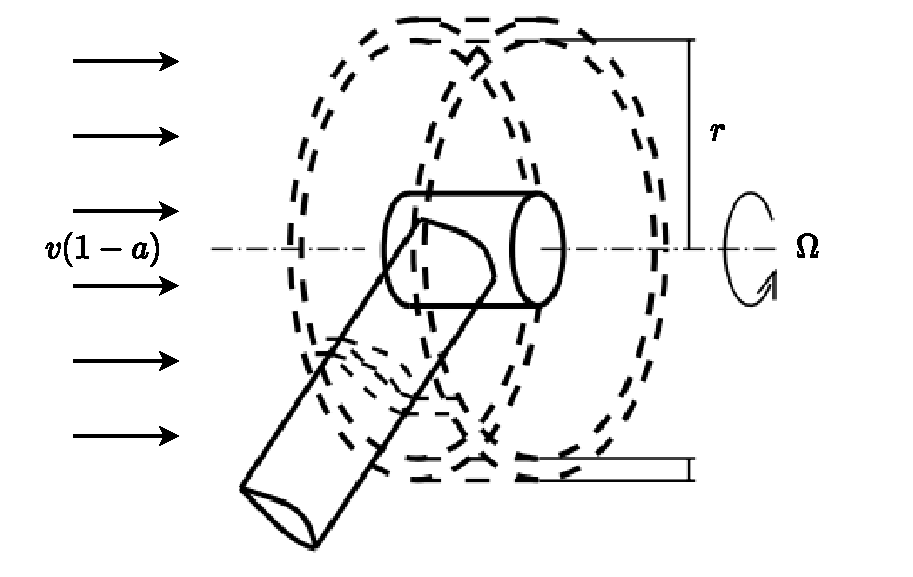
\includegraphics[width=.44\textwidth]{Graphics/RotorBladeElement.pdf}%
		\label{fig:blade_vel_triangles}}
	\hfil
	\subfloat[Velocity triangle]{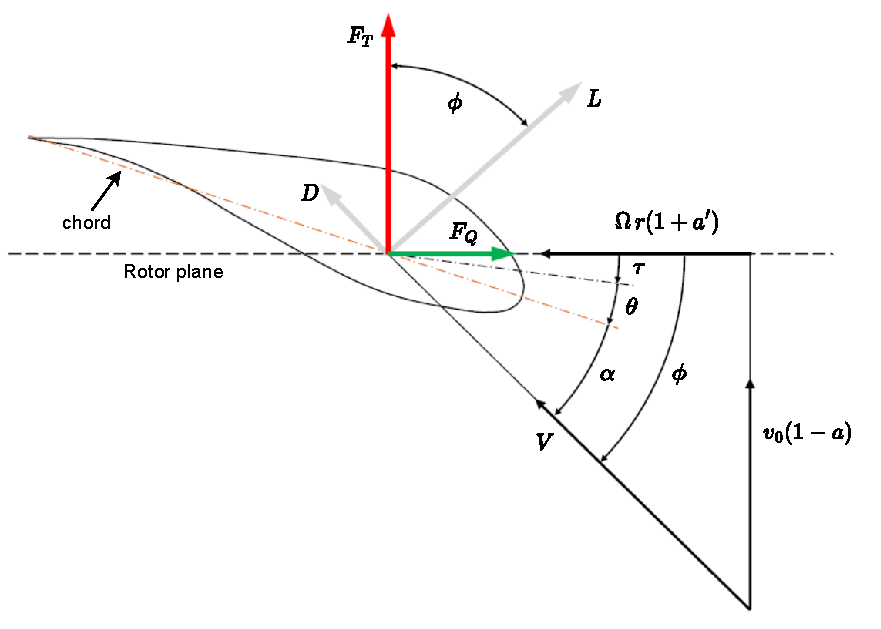
\includegraphics[width=.55\textwidth]{Graphics/BladeVelocityTriangle.pdf}%
		\label{fig:blade_vel_triangle}}
	\caption{Illustrations of a blade cross section and a velocity triangle on a blade section; \textbf{(a)} the blade cross section is made at some distance $ r $ from rotor center and rotates at a frequency $ \Omega $; \textbf{(b)} the velocity triangle acting on a cross section of a WT blade}
	\label{fig:blade_triangles}
\end{figure*}

The resulting wind speed is V with an \textit{inflow angle} $ \phi $. $ F_L $ and $ F_D $ are the lift and drag forces on the blade element respectively. They are calculated from \cref{eq:lift} and \cref{eq:drag}. They include the \textit{chord length} $ c $ which is the length from the leading to the trailing edge of the blade.
\begin{align}
	F_L &= \dfrac{1}{2}\,  \rho \, V^2 c \, C_L \label{eq:lift}\\
	F_D &= \dfrac{1}{2} \, \rho \, V^2 c \, C_D \label{eq:drag}
\end{align}
The lift and drag coefficients $ C_L $ and $ C_D $ are usually extracted from table lookups which are typically found from blade simulations. In a typical scenario $ C_L $ and $ C_D $ are based on the angle of attack $ \alpha $ which is the pitch angle subtracted form the inflow angle: $ \alpha = \phi - \theta $.

The thrust vector $ F_T $ and torque vector $ F_Q $ are then calculated for each blade element from the Pythagorean theorem as in \cref{eq:thrust} and \cref{eq:torque}
\begin{align}
	F_T &= L \, cos(\phi) + D \, sin(\phi) \label{eq:thrust} \\
	F_Q &= L \, sin(\phi) - D \, cos(\phi) \label{eq:torque}
\end{align}
The total thrust and torque of a blade can then be calculated by integrating the above over the length of the rotor blade \cite{Knudsen2013}.


\subsection{Wind turbine control} \label{sec:theory_ctrl}
This section includes a walk-through of the main principles of WT control. A standard WT control scheme is explained with regards to different operation regions. Besides the main controller additional filters and controllers are implemented in the wind industry which mean to improve turbine performance, stability and safety. In this report only the main controller is included.
\begin{figure}[ht]
	\centering
	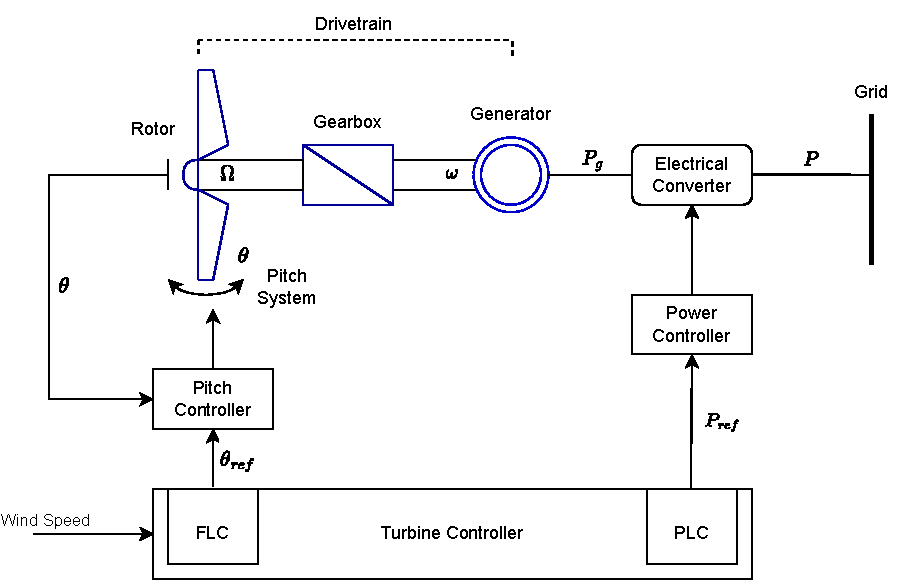
\includegraphics[width=0.7\linewidth]{Graphics/PLC_PI.pdf}
	\caption{An overview of the PLC/FLC controller setup. The turbine controller contains the FLC and PLC which give a pitch reference to the pitch controller and a power reference to the power controller respectively.}
	\label{fig:controller_overview}
\end{figure}
%\medskip
In figure \cref{fig:controller_overview} a simplified illustration is seen of the Vestas controller setup. It yields an overview of the main controllers that handle rotor/generator speed control and power control. The following section is focused on the responsibility of the partial load controller (PLC) and the full load controller (FLC). The depicted "Pitch Controller" and "Power Controller" of the diagram are black boxes from the point of view of this report. They are expected to follow their reference fast enough that it is irrelevant to consider their dynamics.

While the model and controller derived later in this report are designed for the FLC region, a description of the PLC regions and controller is included none the less. It is deemed necessary to understand these to at the very least explain some behaviour of the WT when results are presented later.

A PLC controller can either be specified to output a torque or power reference and each method has advantages and disadvantages. Vestas' controller outputs a power reference. For full scale converter turbines all of the power delivery from the generator to the grid is handled by the electrical converter. The power reference $ P_{ref} $ output by the PLC sets the generator power $ P_g $ by means of the Power Controller.


\subsubsection{Control regions} \label{sec:theory_ctrl_regions}
Wind turbine control can be split into two main stages of control: PLC and FLC. PLC can be further split into three subregions. PLC is related to wind speeds between cut-in wind speed and rated wind speed. In all three PLC regions the generator power or torque reference is regulated based on a generator speed set-point to achieve the most optimal power output. The FLC region is related to the wind speed range from above rated to cut-out wind speed. In this region the pitch angle reference is regulated to track a constant rotor speed and generator power reference. Furthermore each of the four regions are associated with a specific wind speed range. A visualization of these operating regions can be found in figure \cref{fig:operating_regions}. The figure is simply illustrative and especially the width of the regions are out of proportion. 
\begin{figure}[ht]
	\centering
	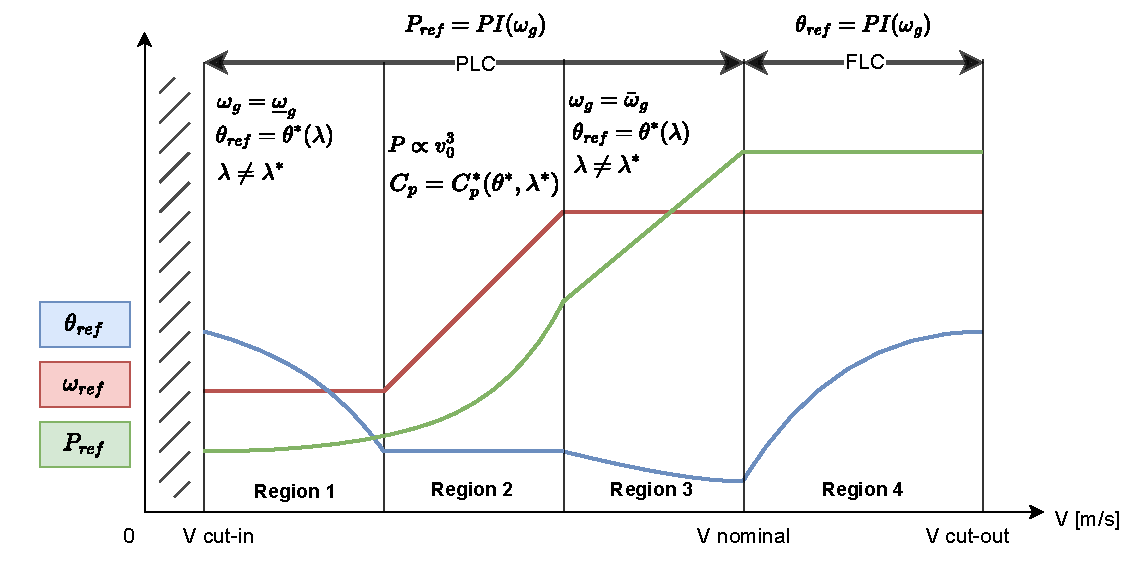
\includegraphics[width=0.9\linewidth]{Graphics/OperatingRegions.pdf}
	\caption{A visualisation of wind turbine control operating regions. Specific wind speeds are not included since these are turbine specific. The figure is illustrative and not correctly scaled.}
	\label{fig:operating_regions}
\end{figure}

%\newpage
Below is a short description of the four regions focused on the parameters which are relevant to the control objective which is firstly maximisation of the turbine power output (PLC) and secondly limitation of the power output to nominal power (FLC).
\begin{itemize}
	\item In \textbf{Region 1} the generator power is regulated to track the minimum rotor speed. The pitch angle reference is set to the optimal angle based on the tip speed ratio which in this region is \underline{not} optimal, meaning that $ C_p \neq C_p^* $. 
	\item In \textbf{Region 2} the pitch angle reference is set to the optimal angle. The tip speed ratio is optimal based on the generator speed which is controlled to the optimal value by means of the generator power. The rotor speed is proportional to the wind speed and power output of the turbine is proportional to the third power of the wind speed. This is intuitive given \cref{eq:power_w_Cp} which shows wind speed to the power three.
	\item In \textbf{Region 3} the generator power is regulated to track the maximum rotor speed. Like in region 1 the pitch angle is set to the optimal angle based on the tip speed which is not optimal.
	\item In \textbf{Region 4} the pitch angle reference is no longer set at an optimal value. It is now set by the FLC PI controller which tracks a constant nominal rotor speed reference. In FLC the power output and rotor speed is ideally constant while the pitch angle is regulated to counteract changes in wind speed.
\end{itemize}



\subsubsection{Partial load control} \label{sec:theory_ctrl_plc}
PLC is active from cut-in wind speed to nominal wind speed. The highest priority of the \textbf{region 2} controller is to maximize $ C_p $ such that $ C_p(\, \lambda) = C_p^*(\theta^*, \lambda^*) $. When observing a 3D plot of $ C_p(\theta, \lambda) $ such as the one in \cref{fig:cp_plot3d} it becomes apparent that maximisation of $ C_p $ will occur for specific values of $ \theta $ and $ \lambda $. In \cref{fig:cp_plot2d} the 3D plot is seen from above and thus only colours are indicators of the size of $ C_p $. Black lines are drawn on the plot which indicate a typical path from cut-in wind speed to cut-out wind speed starting in the top left corner where the tip speed ratio is very high due to the proportionally big difference between the minimum rotor speed and the low incoming wind speed and ending in the bottom right corner with the very high pitch angle. Furthermore the operating regions are drawn along the lines. It becomes obvious that all of region 2 is centred at $ C_p^*(\theta^*, \lambda^*) $ which is marked by a black dot in the middle of the darkest red region. It could be noted from the black line running from region 1 to 3 that it traverses the slope of $ C_p $ which yields the highest $ C_p $ at any given $ \lambda $ such that $ C_p = C_p(\theta^*, \lambda) $.
\begin{figure*}[ht]
	\centering
	
	\subfloat[$ C_p $ vs. $ \theta $ and $ \lambda $ (3D)]
	{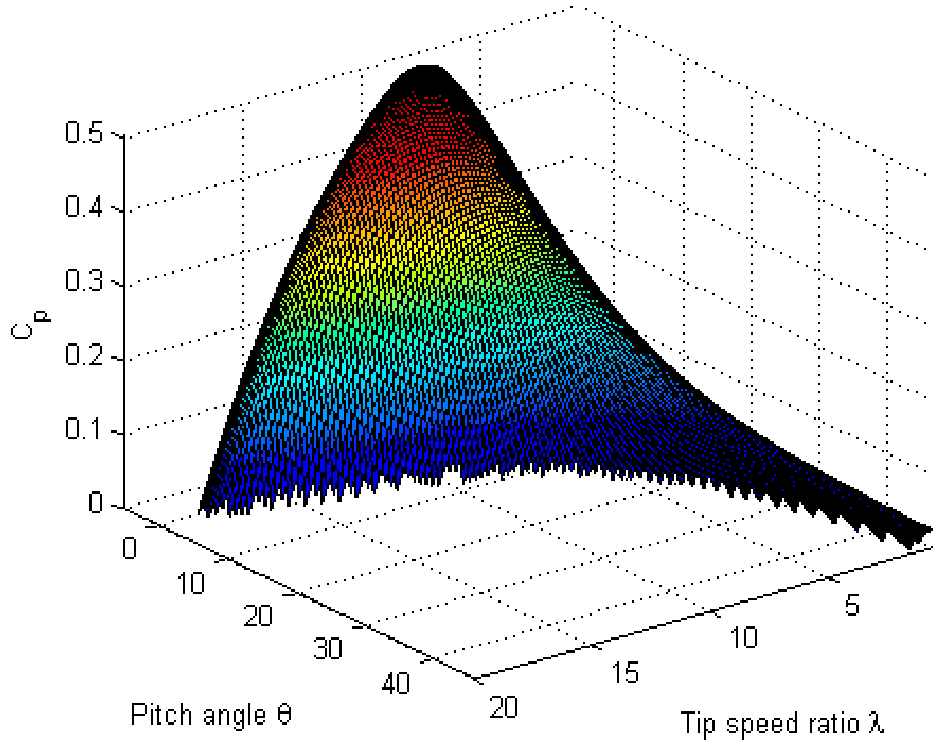
\includegraphics[width=.53\textwidth]{Graphics/Cp3dPlotV2.png}%
		\label{fig:cp_plot3d}}
	\hfil
	\subfloat[$ C_p $ vs. $ \theta $ and $ \lambda $ (2D)]
	{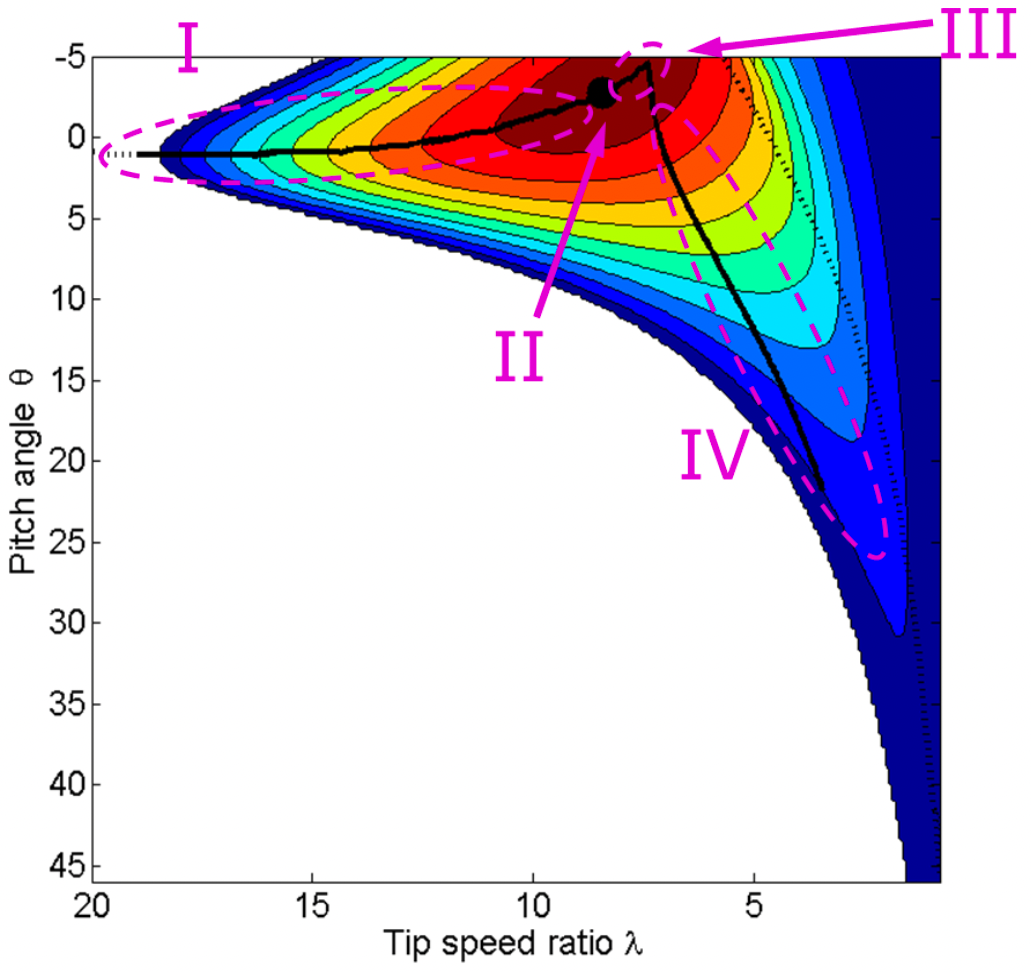
\includegraphics[width=.42\textwidth]{Graphics/Cp2dPlotRegions.png}%
		\label{fig:cp_plot2d}}
	
	\caption{A $ C_p $ plot drawn agains varying $ \theta $ and $ \lambda $; \textbf{(a)} 3D plot; \textbf{(b)} 2D plot where the operating regions are illustrated. Blue signifies low $ C_p $ and red signifies high $ C_p $. Figures are from internal LaC department material.}
	\label{fig:cp_plot}
\end{figure*}

$ \theta $ is determined from table lookups based on $ \lambda $ and thus cannot be utilized as an actuator to control the rotor speed such that $ \lambda(v_0, \Omega) = \lambda^*(v_0, \Omega^*) $ but the generator power can. Thus the primary concern is setting the generator power such that the rotor speed speed is optimal in relation to the wind speed. The rotor speed can in simplified form be described as in \cref{eq:rotor_speed_deriv}. The rotor speed increases when $ T_r > T_g $ and decreases when $ T_g > T_r $.
\begin{equation}\label{eq:rotor_speed_deriv}
	\dot{\Omega} = \dfrac{1}{J} \left( T_r(\theta, v_0) - T_g(P_g, \omega) \right)
\end{equation}
Here $ J $ is the total inertia of all parts connected to the drivetrain, $ T_r $ the rotor torque and $ T_g $ the generator torque referred to the rotor side of the drivetrain. From this equation it becomes apparent that if $ \theta $ is fixed at the optimal angle the generator torque is the only actuator available to control the rotor speed such that $ C_p = C_p^* $.

While there are different generator torque controllers in use in the wind industry the classical WT torque controller is defined as in \cref{eq:gen_torque_ctrl} where a generator torque is calculated based on the rotor speed.
\begin{equation}\label{eq:gen_torque_ctrl}
	T_g = K \Omega^2
\end{equation}
with the \textit{generator constant} being defined like so \cite{Pao2009}:
\begin{equation}\label{eq:gen_torque_const}
	K = \dfrac{1}{2} \rho \pi R^5 \dfrac{C_p^\star}{\lambda^{*3}}
\end{equation}
This causes the rotor speed to tend towards the optimal rotor speed. This is more readily visible when considering \cref{eq:omega_dot}. The equation is derived by combining equations \cref{eq:power2}, \cref{eq:Cp}, \cref{eq:tipspeedratio}, \cref{eq:rotor_speed_deriv} and \cref{eq:gen_torque_ctrl} and \cref{eq:mech_torque}.
\begin{equation}\label{eq:mech_torque}
	T_r = \dfrac{P_T}{\Omega}
\end{equation}
with \cref{eq:mech_torque} simply stating the relationship between mechanical power $ P_T $, rotor speed $ \Omega $ and torque $ T_r $.

For \cref{eq:omega_dot} consider when $ \frac{C_p}{\lambda^3} $ is greater than the optimal counterpart $ \frac{C_p^*}{\lambda^{*3}} $ then $ \dot{\Omega} > 0 $ which will increase $ \Omega $ until an increase in the $ \lambda^3 $ term will bring the two terms closer. $ \theta $ is fixed at $ \theta^* $ and therefore when $ \lambda^3 = \lambda^{*3} $ then $ C_p = C_p^* $ which is exactly the tracking goal.
\begin{equation}\label{eq:omega_dot}
	\dot{\Omega} = \dfrac{1}{2 J} \rho \pi R^5 \Omega^2 \left( \dfrac{C_p}{\lambda^3} - \dfrac{C_p^*}{\lambda^{*3}} \right)
\end{equation}


\medskip
Unlike the conventional torque controller, Vestas utilizes a PI controller structure for its PLC in all three regions. The PI controller input is the generator speed error $ \omega_e $ multiplied with a gain scheduling contribution $ K_{gs}(\omega) $ which depends on the rotor speed:
\begin{equation}\label{eq:pi_plc_ctrl}
	P_{ref} = K_{gs}(\omega) \left(K_{plc,P} \, \omega_e + K_{plc,I} \int \omega_e\right)
\end{equation}
In the simplest case $ K_{gs} = 1/\omega $ and it is included to cancel out the non-linear control authority throughout the operating range of the generator speed.
The generator speed reference in region 2 is calculated from the TSR formula in \cref{eq:tipspeedratio} with $ \lambda = \lambda^* $ like so:
\begin{equation}\label{eq:omega_ref_from_tsr}
	\omega_{ref} = v_0 \dfrac{\lambda^*}{R}
\end{equation} 

In \textbf{region 1} achieving $ C_p = C_p^* $ is disregarded in favour of maintaining a minimum generator speed $ \underline{\omega} $. A minimum rotor speed is implemented to avoid the \textit{blade passing frequency} (3P) overlapping with the eigenfrequency of the system. The 3P frequency is the third multiple of the rotor frequency and this frequency is important with regards to resonance and fatigue loads. An example of a typical cause of 3P resonance is local turbulence streams running through the rotor plane which are struck by each blade - this concept is further explored in \cref{sec:theory_eigenfreq}. As such only $ \theta = \theta^* $ in region 1.

\textbf{Region 3} is characterized by the generator speed reaching nominal speed $ \bar{\omega} $. Thus, like in region 1, optimal $ C_p $ is disregarded to maintain the nominal generator speed. The output  has not reached nominal output power. Thus $ \theta = \theta^* $ and $ P_{ref} $ is regulated to achieve $ \omega = \bar{\omega} $. As the wind increases $ C_p $ decreases while $ P $ increases towards nominal power output. 

The PI controller parameters $ K_{plc,P} $ and $ K_{plc,I} $ are tuned such that satisfactory performance and stability is achieved for a given turbine model. 

As the wind speed reaches the end of region 3 the generator power enters saturation and thus the WT control switches from PLC to FLC which is what the following section is concerned with.


\subsubsection{Full load control} \label{sec:theory_ctrl_flc}
FLC is active from nominal wind speed to cut-out wind speed. The generator speed reference is set to the constant nominal generator speed $ \bar{\omega} $. A PI controller tracks $ \bar{\omega} $ by regulating the collective pitch angle through $ \theta_{ref} $:
\begin{equation}\label{eq:pi_flc_ctrl}
	\theta_{ref} = K_{gs,dP/d\theta} \left(K_{flc,P} \, \omega_e + K_{flc,I} \int \omega_e\right)
\end{equation}
The PI controller output is multiplied with a gain scheduling term to compensate for the pitch-dependent sensitivity $ \frac{dP}{d\theta} $ which results from the non linear pitch authority \cite{Pao2009}. 

The power controller in FLC can be operated at either a constant power or constant torque set-point. Vestas' FLC controller operates with a constant power set-point with varying torque. This is favourable from a grid perspective because a steady power delivery is preferable but as a consequence a negative damping phenomena occurs with regard to the rotor speed. This negative damping phenomena should not be mistaken for the FOWT negative damping problem as they are two separate issues. The negative damping tendency becomes obvious when observing \cref{eq:rotor_speed_deriv} and considering the generator torque:
\begin{equation}\label{eq:gen_torque}
	T_g = \dfrac{P}{\omega}
\end{equation}
If for an example the generator speed decreases then the generator torque increases as a result of maintaining constant power. As a consequence the rotor speed decelerates even further. Consequently the FLC pitch controller must regulate the pitch more actively to compensate for the turbine's increased sensitivity to rotor speed changes.

The FLC PI controller parameters $ K_{flc,P} $ and $ K_{flc,I} $ are tuned such that satisfactory performance and stability is achieved for a given turbine model. 


\subsection{Eigenfrequencies and operating speeds} \label{sec:theory_eigenfreq}
When working with WT control it is relevant to understand the relationship between the \textit{eigenfrequencies} or \textit{modes} of the WT tower and the forces that excite the turbine structure. The eigenfrequency of a system is the frequency at which that system oscillates after an initial disturbance has moved it from its equilibrium position.

A problem that both fixed-bottom and floating WTs have to deal with is frequency separation with regards to the eigenfrequencies of components and the periodic disturbances and exciting forces. Wind and waves will excite the tower at specific frequencies and it is important that such frequencies do not overlap with the turbine modes. If a disturbance such as waves or the wind excite the WT at the same frequency as the eigenfrequency of the tower it will cause the tower to oscillate resulting in an increase in fatigue loads. Therefore towers are designed such that their first and second modes do not overlap with especially the 1P and 3P frequencies. 1P is the rotor rotational frequency and 3P known as the \textit{blade passing frequency} is the third multiple of 1P corresponding to the three blades of conventional horizontal WTs.
\begin{itemize}
	\item \textbf{1P} oscillations typically results from mass imbalance in the rotor blades.
	\item \textbf{3P} oscillations are typically caused by turbulence or wind shear where the wind speed is higher at the rotor top than at the rotor bottom (individual blade pitching is utilized to dampen this effect).
\end{itemize}
\begin{figure}[ht]
	\centering
	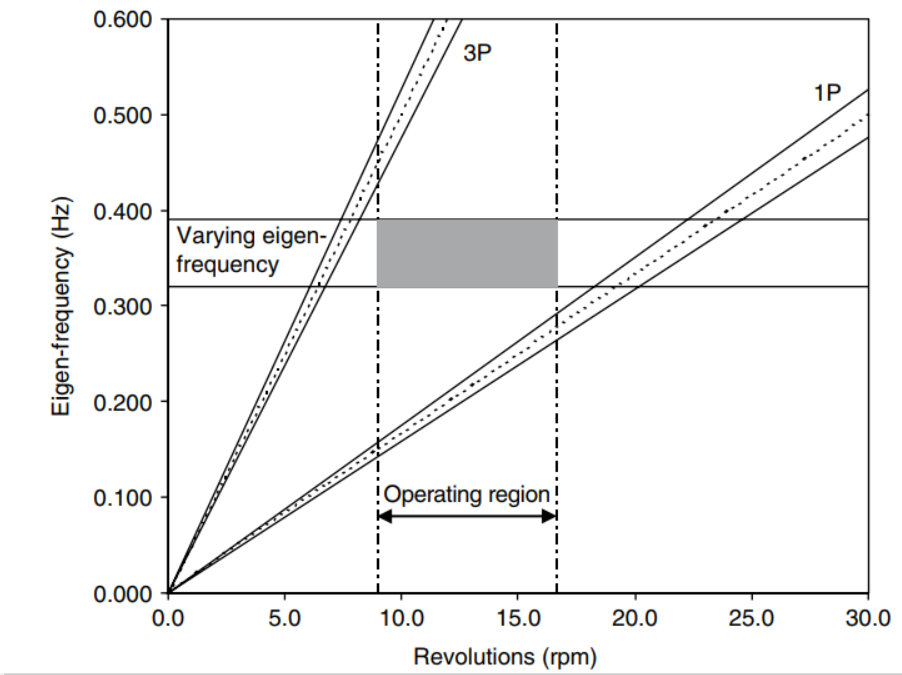
\includegraphics[width=0.5\linewidth]{Graphics/CampbellDiagram.PNG}
	\caption{The Campbell Diagram with the rotation frequency on the x-axis and the eigenfrequency on the y-axis. Figure from \cite{Valentine2015}}
	\label{fig:campbell}
\end{figure}
A Campbell diagram such as the one seen in figure \cref{fig:campbell} is useful for visualizing the relationship between the allowed eigenfrequency of a component and the 1P and 3P frequencies. On the x-axis is the operating frequency of the turbine in revolutions per minute [rpm]. On the y-axis is the eigenfrequency in Hz. Lines are drawn for $ \pm 5 \% $ of both 1P and 3P. For any given turbine the box drawn between the 1P and 3P regions must not touch the lines drawn for the 1P and 3P regions. It becomes apparent why a clear operating region for the turbine rotor speed is defined. For a tower whose operating region is situated between 1P and 3P: If the lower boundary of the rotational speed is lowered the allowable eigenfrequency range decreases. At some point the operating region will have to cross the 1P lines which as explained will cause resonance and as a result increased fatigue loads \cite{Valentine2015}.

\begin{figure}[ht]
	\centering
	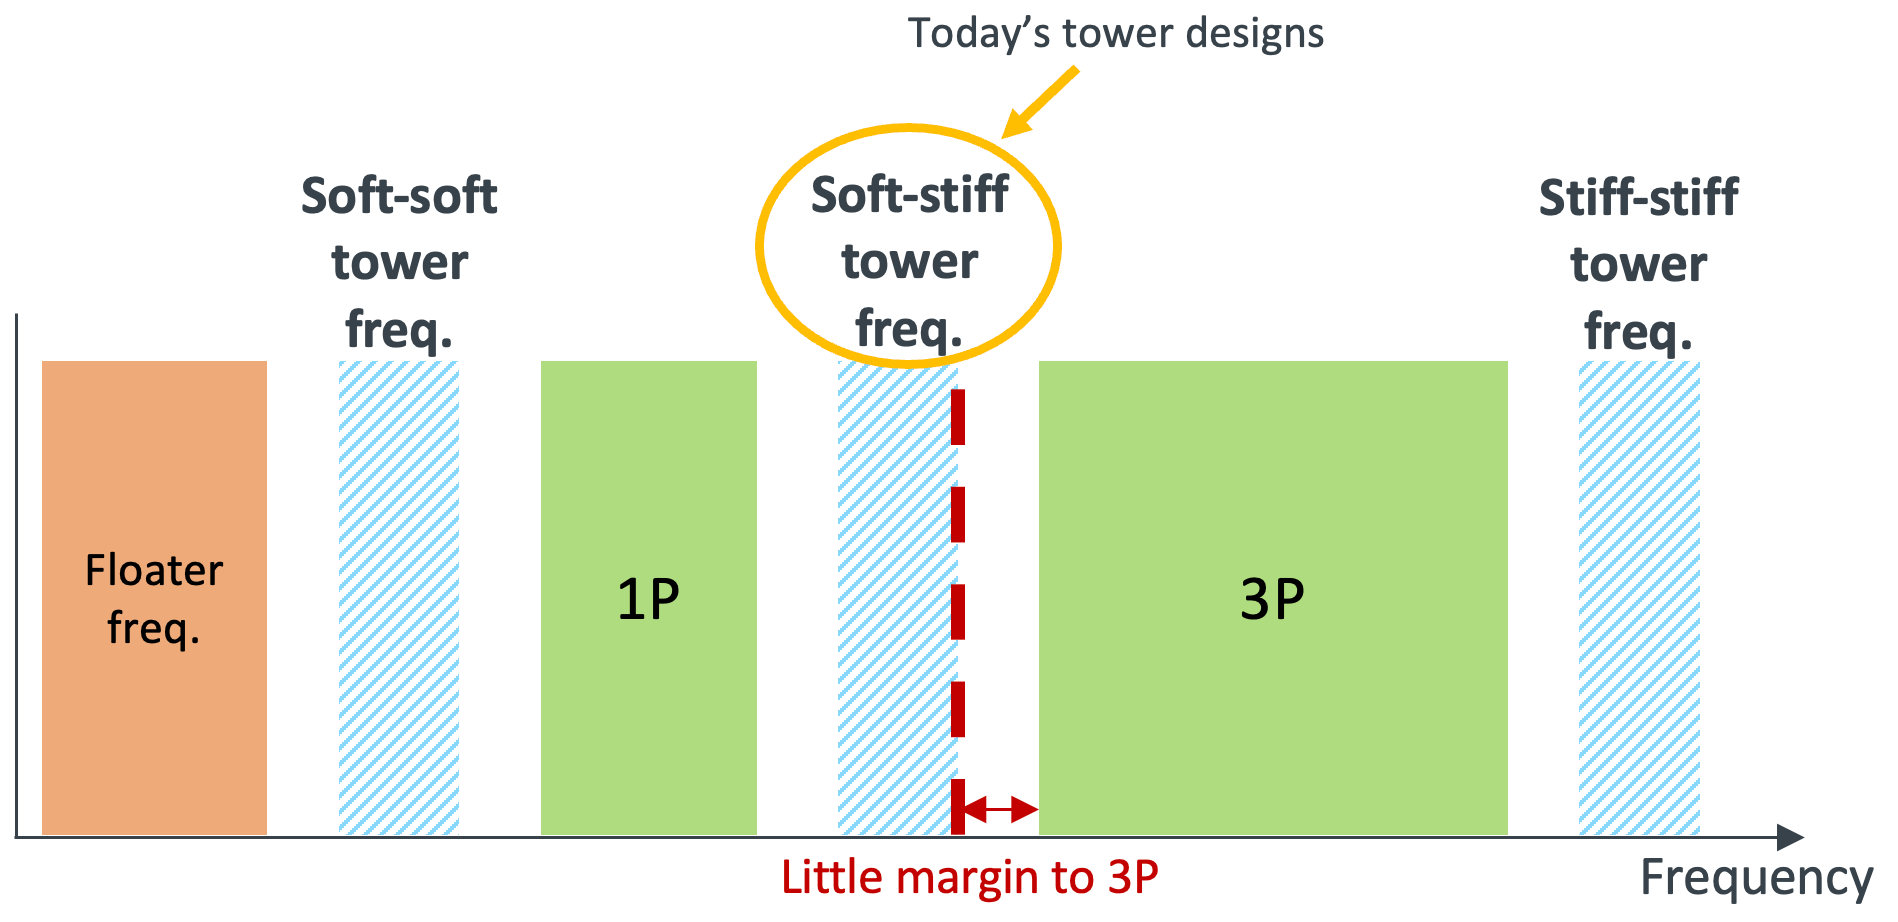
\includegraphics[width=0.7\linewidth]{Graphics/1Pand3PvsTwrStiff.PNG}
	\caption{Illustration of the frequency ranges of tower modes with different tower designs. The floating turbine frequency range is also depicted along with the 1P and 3P frequency ranges. Figure is from internal LaC department material made by Thea Vanelli.}
	\label{fig:1p_and3p}
\end{figure}
Some literature such as \cite{Dykes2018} denote tower designs as \textit{soft-soft}, \textit{soft-stiff} or \textit{stiff-stiff} depending on the position of the first tower eigenfrequency with regards to the 1P and 3P frequencies. Modern WT towers with a \textit{soft-stiff} tower design are made such that their first eigenfrequency ends up between the 1P and 3P and the second eigenfrequency ends up above the 3P frequency. As illustrated in the Campbell Diagram due to varying rotational frequency both 1P and 3P cover a range of frequencies. This is further illustrated in \cref{fig:1p_and3p} which furthermore highlights the possible eigenfrequency ranges of tower designs. In the diagram the eigenfrequency of a FOWTs can be observed in frequencies way lower than 1P. The dotted line just below the 3P frequency resembles the approximate location of the second tower mode. Its location close to 3P can cause unwanted resonance.

\newpage
In \cref{fig:eigen_and_1p3p} an illustration of the tower modes of both fixed-bottom and floating WTs is found. It is apparent that the first tower mode in a conventional fixed-bottom turbine is due to the flexion of the tower while in the floating structure it is due to the tilting of the foundation.
\begin{figure}[ht]
	\centering
	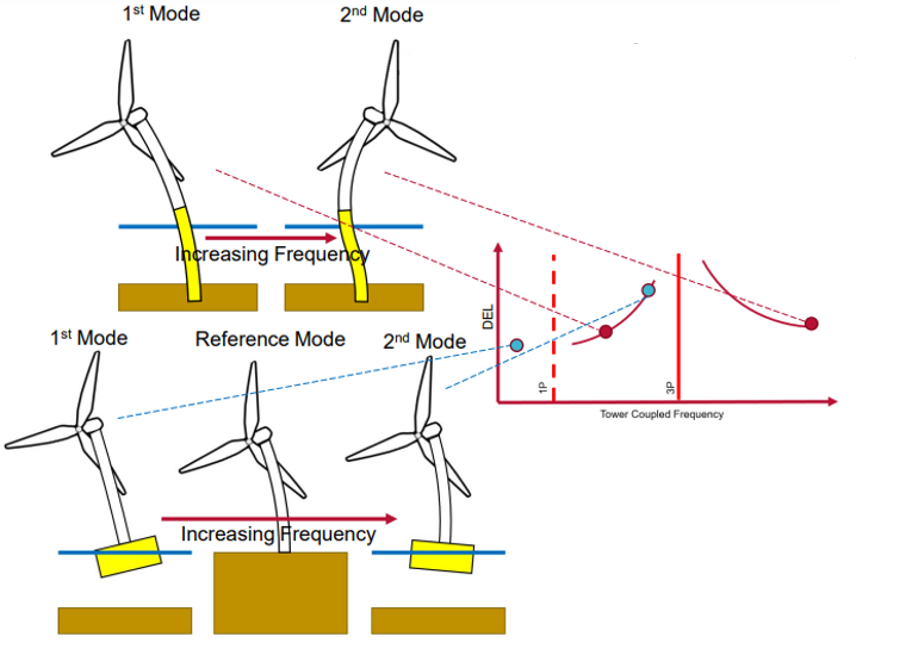
\includegraphics[width=0.6\linewidth]{Graphics/1P3PandEigenFloater.png}
	\caption{Illustration of the 1st and 2nd tower mode of both fixed-bottom and floater turbines. The 1st mode of the floating turbine is lowered down way past the 1P frequency. Figure is from internal LaC department material made by Thea Vanelli.}
	\label{fig:eigen_and_1p3p}
\end{figure}
The oscillations that a FOWT will inevitably experience as a result of both 1P and 3P as well as the fore-aft motion, will result in \textit{fatigue loads} experienced by parts of the turbine. Large fatigue loads can cause damage to components and are therefore relevant to consider - especially in the context of fore-aft motion damping. Thus they are further explained in the following section.


\newpage
\subsection{Fatigue Loads}
The motivation for dampening the fore-aft motion is mainly to reduce loads on the turbine structure while ensuring proper rotor speed tracking. During a WTs lifetime its blades, tower and other components will experience stress mainly in the form of bending due to gravity and the wind. Different materials have different properties which make them able to sustain varying degrees of absolute and cyclic stress. If a component such as a WT blade is subjected to large absolute stress in the form of bending it can be damaged through deformation. The blade's ability to sustain a large degree of bending is largely dependent on the material it is made of. Alternatively the blade can also be damaged by being subjected to many smaller absolute stresses (load cycles) called \textit{cyclic loads} or \textit{fatigue loads}. Again the material defines how many cyclic loads of a given amplitude a component can handle before it is damaged. \textit{Wöhler curves} describe how many cycles of a given amplitude a material can handle before damage occurs and such curves can be seen in \cref{fig:woher_curve}. Some materials will break after a certain number of cycles no matter the stress amplitude but steel has a threshold stress amplitude which in theory means that it can sustain an infinite amount of cycles if the stress amplitude is below said threshold value.

\begin{figure}[ht]
	\centering
	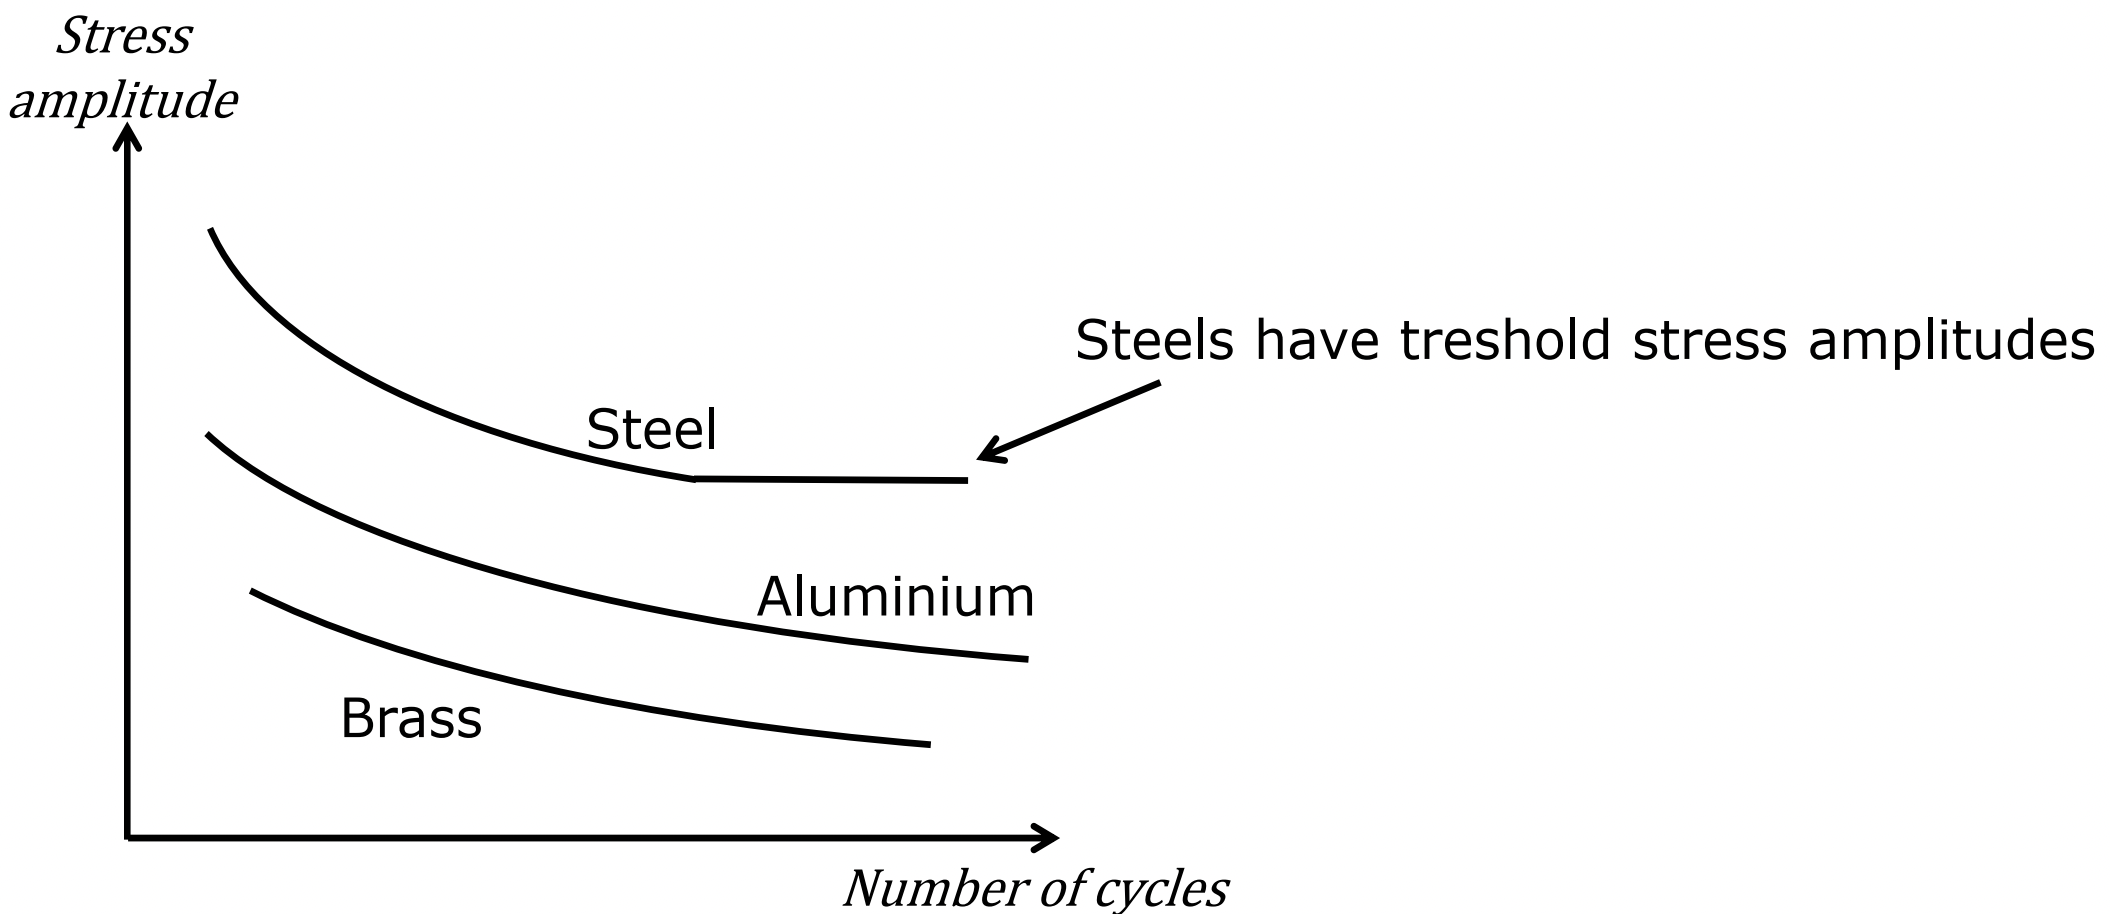
\includegraphics[width=0.6\linewidth]{Graphics/WohlerCurve.png}
	\caption{Illustration of the Wöhler curves of different materials. The curves are only illustrative and not necessarily accurately scaled with respect to each other.}
	\label{fig:woher_curve}
\end{figure}

But of course the amplitude and frequency of cyclic loads experienced by WT components vary in size making it hard to determine when a component might have experienced a specific amount of cyclic loads of a specific amplitude. An equivalent fatigue load of specific frequency and amplitude can be approximated from a set of data to handle this issue called \textit{damage equivalent load} (DEL). DEL can be calculated from the following formula:
\begin{equation}\label{eq:del}
	L_{DEL} = \left( \dfrac{\sum_{i}^{k}n_i L_i^m}{N_{eq}} \right)^{\frac{1}{m}}
\end{equation}
$ k $, $ n_i $ and $ L_i $ are the product of running a set of data from for an example a tower bending moment sensor through an algorithm called \textit{rain flow counting}. Described briefly rain flow counting is a process of defining the cycles and the ranges of these cycles based on data. A given cycle is either a full or half-cycle depending on whether the stress of the material changes direction fully or partly when oscillating. The resulting output is a list of $ k $ amount of cycles which are either full or half cycles $ n_i $ with ranges $ L_i $. The DEL is is then calculated based on the specific material which has a \textit{Wöhler constant} $ m $. It is also dependent on what frequency of oscillation the equivalent fatigue load has and is included in the formula as such:
\begin{equation}\label{key}
	N_{eq} = \dfrac{T_{data}}{T_{eq}}
\end{equation} 
where $ T_{eq} $ is the equivalent fatigue load period and $ T_{data} $ is the time length of the data.

Thus a resulting sinusoid of frequency $ f_{eq} $ and amplitude $ L_{DEL} $ is calculated and can be used to estimate how long a component can sustain loads based on the Wöhler curves. It can also be used to compare the relative reduction of cyclic loads on a component which is the use case in this report.


%\clearpage \newpage
\subsection{FOWT challenges and control} \label{sec:theory_fowt_challenges}
This section is concerned with the challenges that are prevalent in FOWT design and control. In the introduction of the FOWT in \cref{sec:intro_theFOWT} a specific issue; the negative dampening problem, was briefly described. This phenomena is further explored here and other relevant challenges are furthermore touched upon. Lastly a few solutions to the negative dampening problem are briefly presented.

\smallskip
To get a better understanding of the negative damping problem \cref{fig:thrust_vs_windspeed} is considered. It shows the relationship between wind speed and rotor thrust during operation where the turbine controller is active. The specific curve is from the IEA 15 MW reference wind turbine which is the subject of discussion in \cite{Vanelli2021}. The general shape of the curve is not turbine specific for modern turbines. The curve is a product of the relationship between pitch angle, wind speed and rotor speed which is regulated by the WT controller:
\begin{equation} \label{eq:aero_thrust}
	F_T(\theta, \Omega, v) = \dfrac{1}{2} \rho A_d v^2 C_T(\theta, \Omega, v)
\end{equation}
$ C_T $ is the thrust coefficient. In \cref{sec:theory_aero} the rotor thrust was defined for a blade from integrating over the thrust component of each blade element based on a combination of the lift and drag forces. When calculating the total stationary thrust it is convenient to use the pre-calculated thrust coefficient values $ C_T $ to determine the thrust \cite{Knudsen2013}. From \cref{eq:aero_thrust} the rotor thrust's dependency on $ v $ is obvious because of the $ v^2 $ term. The thrust's sensitivity to rotor speed and and pitch angle can only be inferred from the thrust coefficient's sensitivities to said variables. 
\begin{figure}[ht]
	\centering
	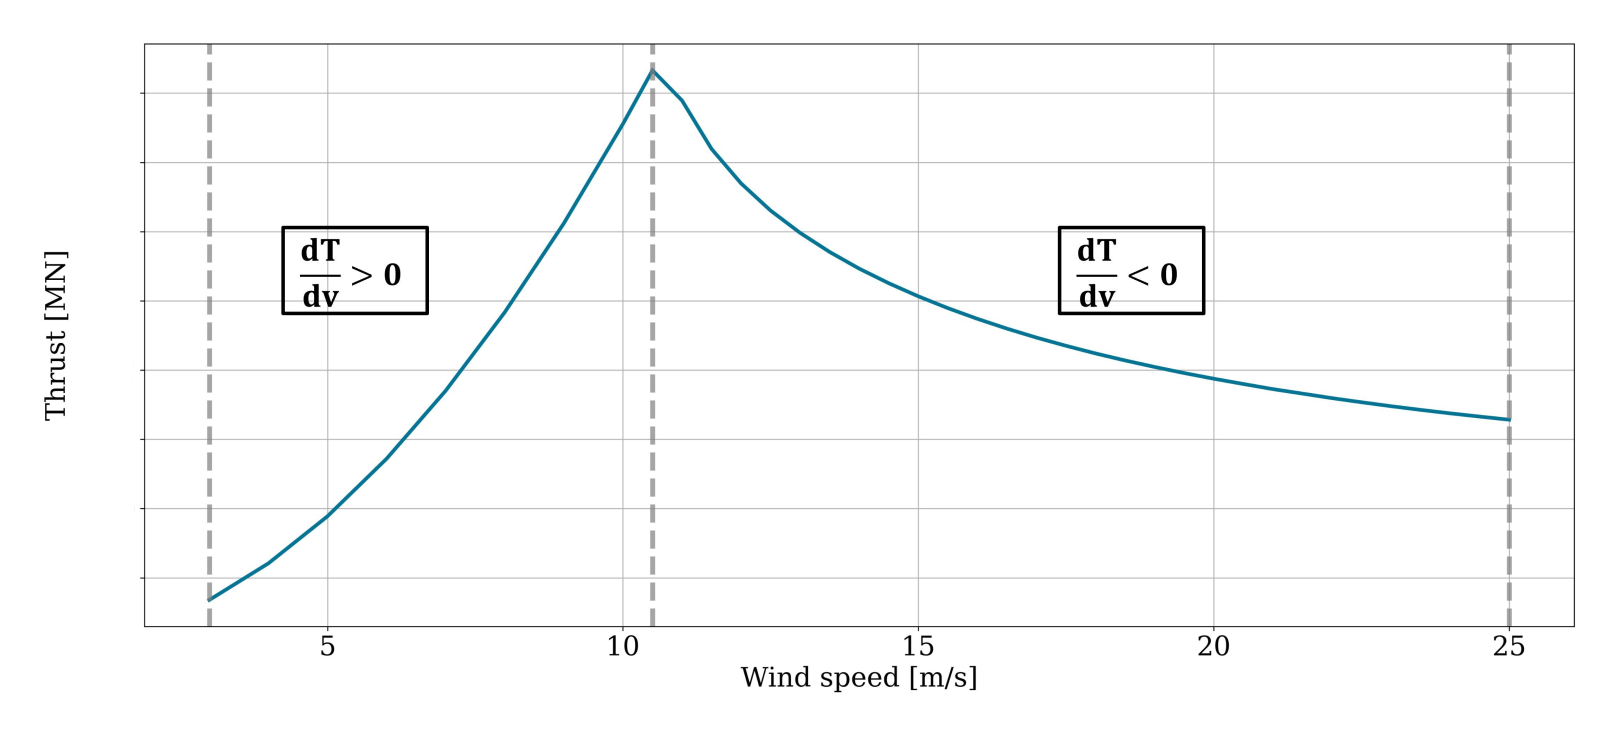
\includegraphics[width=0.85\linewidth]{Graphics/ThrustWindpeedCurve.PNG}
	\caption{Rotor thrust as a function of wind speed for the IEA 15 MW reference wind turbine. Figure from \cite{Vanelli2021}.}
	\label{fig:thrust_vs_windspeed}
\end{figure}
In \cref{fig:thrust_vs_windspeed} it is evident that rotor thrust increases until nominal after which the thrust decreases rapidly again. The increase in thrust before nominal is a product of the increased wind speed and the pitch angle which is either constant or decreasing in PLC as observed in \cref{fig:operating_regions}. An increase in wind speed always yields greater thrust and the FLC keeps the rotor speed constant. Thus the drop in thrust after nominal is due to the FLC increasing the pitch angle to limit the generator power.

% In most of the operating range $ \dfrac{\partial C_T}{\partial \theta} < 0 $ something something.
The wind speed seen by the rotor is a function of the free wind speed and the fore-aft motion: $ v = v_0 - v_y $. $ v_y $ is the velocity of the nacelle in the surge direction and a \textit{backwards motion} refers to a positive movement in this direction. Consider a given wind speed in FLC: If the turbine moves backwards, $ v_y $ increases, resulting in a lowered wind speed $ v $ seen by the rotor. When observing \cref{fig:thrust_vs_windspeed} it is obvious that the thrust increases for lower wind speed. This causes the turbine to move backwards even faster. In the other scenario when the turbine moves forward the wind speed seen by the rotor increases, resulting in an even lower thrust, causing the turbine to move forward with even less resistance. If not properly addressed the result of this behaviour is instability or \textbf{marginal stability}. The test journal in the appendix in \cref{app:tj_02} documented the oscillations resulting from normal FLC operation without a fore-aft motion mitigation strategy. At average wind speeds of 14 m/s and 16 m/s the tower top position velocity oscillates between around -2.2 and 2.2 m/s with a period of around 30 seconds as clearly observed in \cref{fig:tj02_uykf_to_pi1}.

This phenomena is present in both fixed bottom and floating WTs but the problem is greatly exacerbated for FOWTs due to their extra degrees of freedom. For fixed bottom turbines a solution is to detune the controller bandwidth below the system's first eigenfrequency For a fixed-bottom turbine with a reasonably high frequency 1st mode the resulting control performance is usually satisfactory. Vestas' solution is their fore-aft tower damper (FATD) controller addition. In the simplest case the FATD takes the nacelle's horizontal acceleration in the surge direction as input and outputs a collective pitch angle contribution $ \theta_{FATD} $ which is added to the pitch reference:
\begin{equation}\label{eq:fatd}
	\theta_{ref} = \theta_{flc} + \theta_{fatd}
\end{equation}
If the same fore-aft motion mitigation strategies used for fixed bottom WTs are used for floating turbines severe instability issues can ensue \cite{Larsen2007}. Therefore another strategy or tuning must be adopted to handle the negative damping problem on floating turbines. Several solutions are known with the simplest being to detune the FLC to below the first eigenfrequency of the FOWT. While it solves the problem it is a poor solution yielding big rotor speed variations as a result of the very slow rotor speed controller. Other common methods include feeding back the tower top velocity or acceleration through filters to a PI controller which outputs a pitch reference contribution \cite{Grant2022}. Vestas adopts a variation of this method which is simply a heavily detuned version of their FATD. As it stands, tuning of the FATD is mostly trail and error and does not rely on a model.

\smallskip
Furthermore as mentioned in \cref{sec:theory_ctrl_flc} constant power control results in a negative damping term with regards to the rotor speed. This plays an important role for stability since this strategy can result in over-speeding of the rotor in FOWTs. While the constant torque strategy seems to limit the rotor speed variation the improvement comes at the expense of some generator overloading due to the power increasing with rotor speed \cite{Jonkman2010}. As mentioned Vestas utilizes constant power tracking and thus this strategy is assumed in this project.